\documentclass[border=0.5cm]{standalone}
\usepackage{tikz}
\definecolor{brightpink}{rgb}{1.0, 0.0, 0.5}
\definecolor{brightgreen}{rgb}{0.4, 1.0, 0.0}
\definecolor{caribbeangreen}{rgb}{0.66, 0.89, 0.63}
\begin{document}

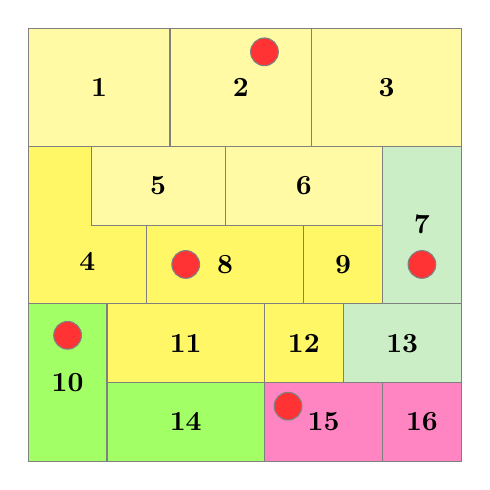
\begin{tikzpicture}[thin,draw=gray,font=\bf,fill opacity=0.6, text opacity=1]
\draw[fill=brightgreen] (0,0) rectangle (1,2)node[midway]{10};
\draw[fill=brightgreen] (1,0) rectangle (3,1)node[midway]{14};
\draw[fill=brightpink!80] (3,0) rectangle (4.5,1)node[midway]{15};
\draw[fill=brightpink!80] (4.5,0) rectangle (5.5,1)node[midway]{16};
\draw[fill=yellow] (1,1) rectangle (3,2)node[midway]{11};
\draw[fill=yellow] (3,1) rectangle (4,2)node[midway]{12};
\draw[fill=caribbeangreen] (4,1) rectangle (5.5,2)node[midway]{13};
\draw[fill=caribbeangreen] (4.5,2) rectangle (5.5,4)node[midway]{7};
\draw[fill=yellow] (3.5,2) rectangle (4.5,3)node[midway]{9};
\draw[fill=yellow] (1.5,2) rectangle (3.5,3)node[midway]{8};
\draw[fill=yellow] (0,2) -- (1.5,2)node[midway,above=0.3cm]{4} -- (1.5,3) -- (0.8,3) -- (0.8,4) -| cycle;
\draw[fill=yellow!60] (0.8,3) rectangle (2.5,4)node[midway]{5};
\draw[fill=yellow!60] (2.5,3) rectangle (4.5,4)node[midway]{6};
\draw[fill=yellow!60] (0,4) rectangle (1.8,5.5)node[midway]{1};
\draw[fill=yellow!60] (1.8,4) rectangle (3.6,5.5)node[midway]{2};
\draw[fill=yellow!60] (3.6,4) rectangle (5.5,5.5) node[midway]{3};

% Circles
\draw [fill=red!80,opacity=1] (0.5,1.6) circle(5pt);
\draw [fill=red!80,opacity=1] (3.3,0.7) circle(5pt);
\draw [fill=red!80,opacity=1] (5,2.5) circle(5pt);
\draw [fill=red!80,opacity=1] (2,2.5) circle(5pt);
\draw [fill=red!80,opacity=1] (3,5.2) circle(5pt);


\end{tikzpicture}

\end{document}
